\documentclass[12pt,fleqn]{article}\usepackage{../../common}
\begin{document}
Örneklem Dağılımları (Sampling Distributions)

Bir (ve en önemli) örneklem dağılımını daha önce gördük, ki bu Normal
dağılımdır. $\bar{X} = (X_1 + X_2 + ... + X_n) / n$ ortalaması ortalaması
$\mu$ ve standard sapması $\sigma/n^2$ olan bir Normal dağılıma
yaklaşır. Tabii bu dağılım standardize edilebilir, vs. Fakat rasgele
değişkenler üzerinde pek çok işlem mümkündür, ve bu işlemlerin bazıları
artık ünlü olan yeni / başka dağılımlar ortaya çıkartmışlardır. Bu
dağılımlar önemlidir, çünkü mesela bazı uygulamalarda veri noktalarının
karesini alırız, ve bu karesi alınmış normal noktaların bambaşka bir
dağılımı vardır! Bu önemlidir çünkü veri noktalarının normalliği
faraziyesinden hareketle kare alma işlemi gerektiren her ne hesap ise onun
doğruluğunu bu sonuç dağılıma sorarak kontrol edebiliriz! 

Devam edelim. 

$\frac{\bar{Y}-\mu}{\sigma / \sqrt{n}}$ ve $\frac{\bar{Y}-\mu}{S  /\sqrt{n}}$ 
Karşılaştırması

Diyelim ki normal olarak dağıldığını bildiğimiz bir nüfustan $Y_1,..,Y_n$
rasgele örneklemini topladık, ve amacımız bilinmeyen gerçek $\mu$ hakkında
bazı sonuçlara varmak. Eğer varyans $\sigma^2$ biliniyorsa, bu noktadan
sonra ne yapacağımız gayet açık: daha önce gördüğümüz gibi bir karar kuralı
ortaya çıkartmak, ya da güven aralığı hesaplamak çok kolay, ki bu
tekniklerin temelinde $Z = \frac{\bar{Y}-\mu}{\sigma / \sqrt{n}}$ dağılımının standart normal $f_Z(z)$'ye 
yaklaşması yatıyor. 

Fakat pratikte $\sigma^2$ genellikle bilinmez, o zaman nüfus varyansının
tahmin edicisi $S^2 = \frac{1}{n-1}\sum_{i=1}^n (Y_i-\bar{Y})^2$
kullanılır, ki bu maksimum olurluk tahmin edicisinin yansız (unbiased)
versiyonu. Fakat buradaki önemli soru şu: $\sigma^2$ yerine $S^2$ koyma Z
oranını nasıl etkiler? Daha önce büyük örneklemler için bir fark
olmadığından bahsettik. Peki küçük örneklemler için? 

Küçük $n$ için bu iki oranının birbirinden farklı olduğununun keşfi William
Sealy Gossett adlı araştırmacıya ait. 1899'da Oxford'dan Kimya ve Matematik
bölümünden mezun olduktan sonra Gossey, Guiness adlı şirkette çalışmaya
başladı. Ürünlerin üzerinde yapacağı deneylerden aldığı veriler lojistik
bazı sebepler dolaşışıyla çok azdı, ve ``gerçek'' $\sigma^2$'nin bilinmesi
mümkün değildi. Çoğu zaman $n$ 4 ya da 5'den bile az oluyordu. Bu gibi
durumlarla uğraşa uğraşa Gossey $\frac{\bar{Y}-\mu}{S / \sqrt{n}}$'nin
beklendiği gibi çan eğrisi $f_Z(z)$ şeklinde değil, daha ``etekleri
kabarık'' başka bir dağılım gibi gözüktüğünü farketti, yani sıfırdan çok
küçük ya da ondan çok büyük oranların ihtimali çok düşük değildi. 
 
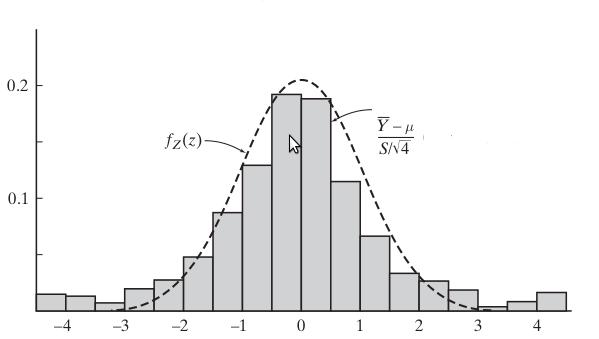
\includegraphics[height=5cm]{stat_sampling_01.png}

Üstteki histogram $S$ kullanarak hesaplanmıştır, $n=4$ olmak üzere 500
deney üzerinden hesap yapılmıştır. İki dağılımın birbirinden uzaklaştığı
görülüyor. 

Genel olarak düşünmek gerekirse, olasılık dağılımları iki büyük kategori
altına düşer. Aşağı yukarı bir düzine kadarı gerçek dünyadan alınabilecek
her ölçümü olduğu haliyle iyi modelleme kabiliyetine sahiptir; mesela
normal, binom, Poisson, üstel dağılımlar gibi. Diğer yandan daha az sayıda
(ama bir o kadar önemli) dağılımlar $n$ tane rasgele değişkenin üzerinden
hesaplanan {\em fonksiyonların} nasıl davrandığını çok iyi modeller. İşte
bu dağılımlara örneklem dağılımları ismi verilir ve tipik kullanım alanları
çıkarsama (inference) yapmaktır.

Normal dağılımı her iki kategoriye de aittir. Hem ayrı ayrı ölçümleri
modellemek, hem de $\frac{\bar{Y}-\mu}{\sigma / \sqrt{n}}$'in olasılıksal
davranışını modellemek için kullanılır.  İkinci kullanımı normal dağılımın
bir örneklem dağılımı olarak kullanılmasına örnektir.

Normal dağılımdan sonra en önemli üç örneklem dağılımı Öğrenci t Dağılımı,
chi kare dağılımı ve F dağılımıdır. Son iki dağılım t oranını temsil eden
$f_T(t)$'yi, yani $T = \frac{\bar{Y}-\mu}{S / \sqrt{n}}$'yi türetmek için
gerekli.

Türetmek 

Şaşırtıcı gelebilir ama t dağılımının yoğunluk fonksiyonunu türetmek pek
kolay bir iş değildir, ilk başta kolay yapılabilirmiş gibi geliyor, çünkü
Merkezi Limit Teorisinin temelini oluşturan $\frac{\bar{Y}-\mu}{\sigma / \sqrt{n}}$'in 
yoğunluğunu türetmek nisbeten basit, moment üreten fonksiyonlar ile
yapılabiliyor. Fakat $\frac{\bar{Y}-\mu}{\sigma / \sqrt{n}}$ 
ifadesinden $\frac{\bar{Y}-\mu}{S / \sqrt{n}}$ ifadesine
geçmek çok daha zor, çünkü bu durumda T {\em iki tane} rasgele değişkeninin
bir oranı haline gelmiştir.

t Dağılımının ispatı için şu basamaklar gerekiyor; Önce standart normal
rasgele değişkenlerin karelerinin toplamının gamma dağılımın özel bir hali
olan chi kare dağılımı olduğunu göstermek. Daha sonra normal dağılmış olan
bir nüfustan alınan $n$ örneklemden elde edilen $\bar{Y}$ ve $S^2$'nin
birbirinden bağımsız rasgele değişkenler olduğunu göstermek, ve
$\frac{n-1}{S^2}$'nin chi kare olarak dağıldığını ispatlamak. Daha sonra
sıra birbirinden bağımsız iki chi kare yoğunluk fonksiyonunun arasındaki
oranı türetmeye gelecek, ki bu bir F dağılımıdır. En son olarak $T^2
=(\frac{\bar{Y}-\mu}{S / \sqrt{n}})^2$ ifadesinin 
birbirinden bağımsız iki chi kare dağılımının oranı olduğunu göstermek ki
$T^2$  ifadesi F dağılımının özel bir halidir.

Chi Kare, $\chi^2$ Dağılımı

Tanım

$Z_1, .. , Z_p$ bağımsız standart Normal rasgele değişkenler ise, $U = \sum_{
  i=1}^{p} Z_p^2$ ki bu dagilima $p$ derecede serbestliğe (değrees of freedom)
olan chi kare dağılımı (chi square distribution, yani $\chi^2$) ismi verilir.

Teori

$U$, $p$ derece serbestliğe sahip bir $\chi^2$ dağılıma sahip ise, ki yoğunluk 

$$
f_U(u;p) = \frac{ 1}{\Gamma(\frac{p}{2}) 2^{p/2}} u^{(p/2) - 1} e^{-u/2} 
$$

$$ u \ge 0 $$

$$ \Gamma(a) = \int_{0}^{\infty} t ^{a-1} e^{-t} \ud t $$

Üstteki yoğunluğun $r=m/2$ ve $\lambda=1/2$ olan bir Gamma dağılımı olduğu
da söylenebilir. Fonksiyonunun parametresi sadece $p$'dir. İspat için [1,
sf. 388].

$$ E[U] = p $$

$$ Var[U] = 2p $$

F Dağılımı

Diyelim ki $U$ ve $V$ birbirinden bağımsız, ve sırasıyla $m$ ve $n$ derece
serbestliğe sahip iki chi kare dağılımı. O zaman $\frac{V/m}{U/n}$ olarak
hesaplanan yeni bir rasgele değişkenin dağılımı, $m,n$ derece serbestliğe
sahip bir F dağılımı olarak ifade edilir.

Teori

Rasgele değişken $\frac{Z^2}{U/n}$, ki $U$ bir chi kare dağılımıdır, 1,n
derece serbestliğe sahip bir F dağılımına sahiptir. 

İspatı burada vermiyoruz.

Teori $\mlabel{1}$

$Y_1,..,Y_n$ ortalaması $\mu$, varyansı $\sigma^2$ olan bir normal dağılımdan
alınan $n$ örneklem olsun. O zaman

a. $S^2$ ve $\bar{Y}$ birbirinden bağımsızdır

b. $\frac{(n-1)S^2}{\sigma^2}=\frac{1}{\sigma^2}\sum_{i=1}^{n}(Y_i-\bar{Y})^2)$
hesabı $n-1$ derece serbestliğe sahip bir chi kare dağılımıdır.

İspat için [1, sf. 388].

Nihayet $\frac{\bar{Y}-\mu}{S / \sqrt{n}}$ ifadesinin yoğunluğunu bulmak için
tüm altyapıya sahibiz.

Tanım

$Z$ bir standart normal rasgele değişken, $U$ ise $n$ derece serbestlikteki
bir chi kare rasgele değişken olsun. O zaman $n$ derece serbestliği olan
Öğrenci t oranı (Student's t ratio)

$$ 
T_n = \frac{Z}{\sqrt{ \frac{U}{n}}} 
\mlabel{2} 
$$

olarak belirtilir.

Teori

$Y_1,..,Y_n$, bir $\mu,\sigma$ normal bir dağılımdan alınmış bir rasgele
örneklem olsun. O zaman 

$$ T_{n-1} = \frac{\bar{Y}-\mu}{S/\sqrt{n}}$$

$n-1$ serbestlik derecesine sahip bir t Dağılımıdır. 

İspat

$\frac{\bar{Y}-\mu}{S/\sqrt{n}}$ ifadesini şu şekilde yazabiliriz, 

$$ \frac{\bar{Y}-\mu}{S/\sqrt{n}} =
\frac{\frac{\bar{Y}-\mu}{\sigma/\sqrt{n}} }
{\sqrt{\frac{(n-1)S^2}{\sigma^2(n-1)}}}
$$

Değil mi? Alttaki karekök içindeki bölendeki $n-1$'ler birbirini iptal
eder, karekök kare ifadelerini iptal eder, ve geriye kalan $S/\sigma$, ters
çevirilip $\sigma/S$ olarak $\frac{\bar{Y}-\mu}{\sigma/\sqrt{n}}$'yi
çarpacaktır, onun bölümdeki $\sigma$'sini iptal edecektir, ve nihai bölüme
$S$ yerleştirilmiş olur, ve eşitliğin solundaki ifadeye erişiriz. Fakat bu
dönüştürücü bölüm ifadesi sayesinde eşitliğin sağ tarafında yeni bir
formüle eriştik; karekök ifadesi içine bakarsak üstteki (b) teorisiyle
uyumlu olarak $\frac{(n-1)S^2}{\sigma^2}$ görüyoruz, ki bu ifade bir chi
kare dağılımı.

Diğer yandan eşitliğin sağındaki bölüm kısmı bir standart normal. Yani
(2)'de tarif edilen duruma erişmiş oluyoruz, üstteki ifade bu tanıma göre
bir t Dağılımı. 

t Dağılımı (Student's t) 

$X$, $n$ derece bağımsızlıkta $t$ dağılımına sahiptir, ve dağılımı

$$ 
f_T(t) = 
\frac
{
\Gamma(\frac{n+1}{2})
}
{
\sqrt{n\pi}\Gamma(\frac{n}{2})
\bigg(1+\frac{t^2}{n}\bigg)^{(n+1)/2}
}
 $$

Aslında Normal dağılımı $t$ dağılımının $v = \infty$ olduğu hale tekabül
eder. Cauchy dağılımı da $t$'nin özel bir halidir, $n = 1$ halidir. Bu
durumda yoğunluk fonksiyonu

$$ f(x)  = \frac{ 1}{\pi(1+ x^2)} $$

Bu formül hakikaten bir yoğunluk mudur? Kontrol için entegralini alalım, 

$$
\int_{ -\infty}^{\infty} f(x) \ud x = 
\frac{ 1}{\pi} \int_{ -\infty}^{\infty} \frac{\ud x}{1 + x^2} 
$$

Çoğunlukla entegre edilen yerde  ``1 artı ya da eksi bir şeyin karesi''
türünde  bir ifade görülürse, yerine geçirme (subsitution) işlemi
trigonometrik  olarak  yapılır. 

$$  x = \tan \theta, \theta = \arctan x $$

$$ 1 + x^2 = 1 + \tan^2\theta = \sec^2\theta$$

$$ dx / d\theta = \sec^2\theta $$

O zaman 

$$ =
\frac{ 1}{\pi} \int_{ -\infty}^{\infty} \frac{\ud x}{1 + x^2}   =
\frac{ 1}{\pi} \int_{ -\infty}^{\infty}  \frac{ 1}{\sec^2\theta}\sec^2\theta \ud\theta = 
\frac{ 1}{\pi} \int_{ -\infty}^{\infty}  1 \ud\theta = 
$$

$$ = 
\frac{ 1}{\pi} \theta |_{ -\infty}^{\infty}   = 
\frac{ 1}{\pi} [\arctan(\infty) - \arctan(-\infty)]
 $$

$$ =
\frac{ 1}{\pi} [\frac{ \pi}{2} - (-\frac{ \pi}{2}) ] = 1
 $$



Kaynaklar

[1] Larsen, {\em Introduction to Mathematical Statistics and Its Applications}

[2] Runger, {\em Applied Statistics and Probability for Engineers}


\end{document}
